\section{Method} \label{sec:method} 

In this section we will describe the method we have used to solve the Authorship
Verification problem presented. In general there are two methods of representing
each author. There is the instance based approach and the profile based
approach. In the instance based approach each author is represented by a set of
texts they have written while in the profile based approach they are represented
by the sum of the set of texts they have written. The instance based approach is
illustrated in Figure \ref{fig:instance_based} and the profile based approach is
illustrated in Figure \ref{fig:profile_based}.

\begin{figure}[htb]
    \centering
    \textbf{Instance Based Authorship Verification or Authorship Attribution}
    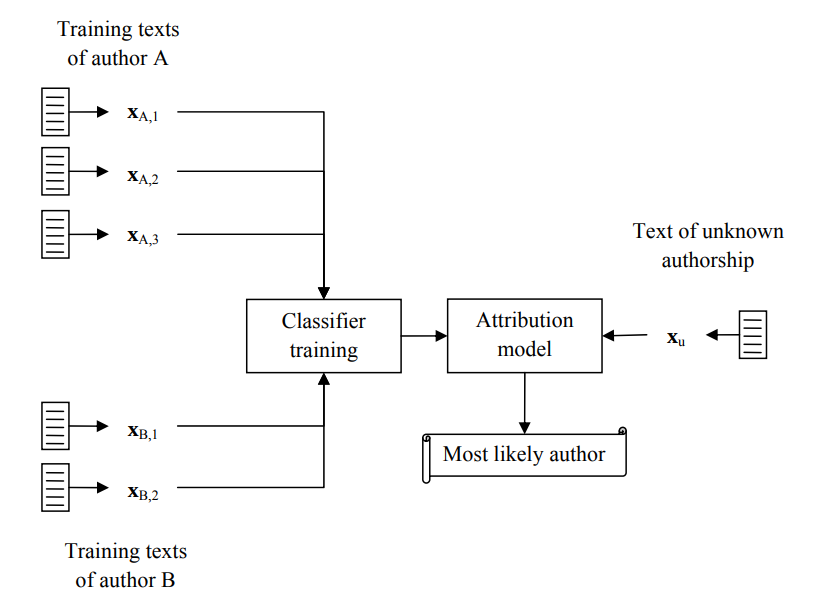
\includegraphics[scale=0.4]{./pictures/method/instance_based.png}

    \caption{Illustrate the typical instance based Authorship Verification or
        Authorship Attribution solution setup.\cite{stamatos2009} A set of
        authors are given as input each with a set of texts. Some Machine
        Learning model is trained on the input texts and the model is used to
        predict an unknown text. In the Authorship Verification case the
        prediction is either "same author" or "different author" while in the
        Authorship Attribution case the prediction will be one of "author 1",
        "author 2", \dots, "author n".}
    \label{fig:instance_based}
\end{figure}

\begin{figure}[htb]
    \centering
    \textbf{Profile Based Authorship Verification or Authorship Attribution}
    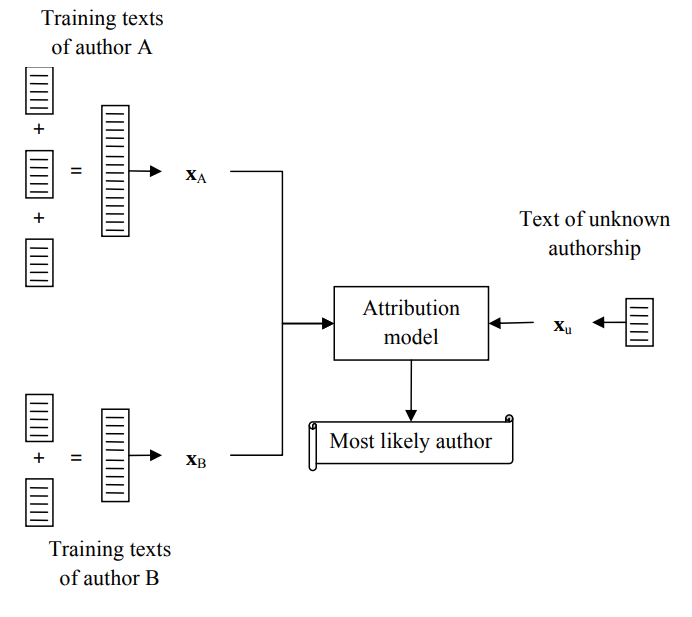
\includegraphics[scale=0.4]{./pictures/method/profile_based.png}
    \caption{Illustrate the typical profile based Authorship Verification or
        Authorship Attribution setup.\cite{stamatos2009} The texts of each
        author are combined using some combination function such as an average
        or concatenation. Those \textit{profiles} are then given to a Machine
        Learning model to train. The output is a model which is used to predict
        unknown texts. If it is the Authorship Verification case the prediction
        output is either "same author" or "different author" and if it is the
        Authorship Attribution case the output is one of "author 1", "author 2",
        \dots, "author n".}
    \label{fig:profile_based}
\end{figure}

We will generally use the instance based approach and we will generally use
Authorship Verification. The reason we use an instance based approach is that
that allows us to use extra information from each single text. For example
writing style may change over time especially for secondary school pupils that
evolve very much in a short amount of time. Since we use an instance based
approach we are able to weight similarity to newer texts higher than similarity
to older texts.

There are also another split between methods that we consider. There are
generalizing and author specific models. In a generalizing model only a single
model is trained on data from multiple authors and are able to make predictions
about third party authors. In the author specific model a separate model has
to be trained for each author and is not able to make predictions for third
party authors. The generalizing model has the advantage that it only has to be
trained once and after that it can be used for everyone. The author specific
model has the advantage that it can better fit to the specific quirks of a
particular author since it is trained separately for each author. The downside
of the author specific approach is that a new model has to be trained for each
new author. We will focus on the generalizing approach since it is easier to
implement for MaCom as they only have to train a model once.

As a unit of measuring the quality of our models, and how well they adhere to
95\% specificity constraint, we will also compute the number of \gls{TP}s,
\gls{TN}s, \gls{FP}s and \gls{FN}s, as was done
in a project previously created by us.\cite{US} In these problems we get,

\begin{itemize}
    \item a \gls{TP} whenever we answer \textit{True} and the texts are written
        by the same author,
    \item a \gls{TN} whenever we answer \textit{False} and the texts are
        \textbf{not} written by the same author,
    \item a \gls{FP} whenever we answer \textit{True} and the texts are
        \textbf{not} written by the same author,
    \item a \gls{FN} whenever we answer \textit{False} and the texts are written
        by the same author.
\end{itemize}

Given those definitions the \gls{TPR}, \gls{FPR}, \gls{TNR} and \gls{FNR}
describes.

\begin{description}
    \item[\gls{TPR}: ] The fraction of positives that we reported \textit{True}
        on i.e. the fraction of texts written by the same author that we say are
        written by the same author.
    \item[\gls{FPR}: ] The fraction of negatives that we reported \textit{True}
        on i.e. the fraction of texts written by different authors that we say
        are written by the same author.
    \item[\gls{TNR}: ] The fraction of negatives that we reported \textit{False}
        on i.e. the fraction of texts written by different authors that we say
        are written by different authors.
    \item[\gls{FNR}: ] The fraction of positives that we reported \textit{False}
        on i.e. the fraction of texts written by the same author that we say are
        written by different authors.
\end{description}

And they can be computed as,

\begin{align}
    TPR &= \frac{TP}{TP + FN}, \\
    FPR &= \frac{FP}{FP + TN}, \\
    TNR &= \frac{TN}{TN + FP}, \\
    FNR &= \frac{FN}{FN + TP}.
\end{align}

In the case of MaCom, we want to minimize the \gls{FNR} as much as possible, so
as to not wrongfully accuse anyone of not having written their assignment.


\subsection{Neural Network Model}

A Neural Network consist of a collection of neurons. Each neuron is a simplified
mathematical model of a neuron in a brain. Each neuron has a set of inputs
called $x_i$ and a single output called $z_i$. The neurons compute a weighted
sum of its inputs and applies an activation function $h$ to the weighted sum.
The weights are called $w_i$. The function each neuron computes is then,

\begin{equation}
    z_i = h\left(
        \sum_{i = 1}^d w_ix_i + w_0
    \right).
\end{equation}

The learning of each neuron consist of changing the weights of the inputs to
give a better output. The activation function $h$ is usually a non linear
function. A plot of different activation functions are shown in Figure
\ref{fig:activation_functions}.

\begin{figure}
    \centering
    \textbf{Activation Functions}\par\medskip
    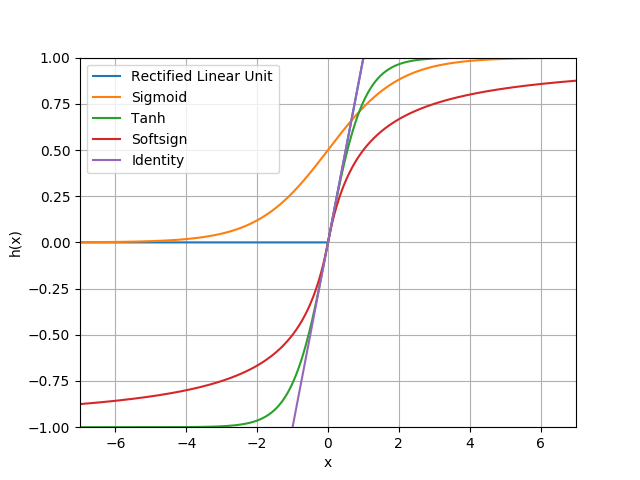
\includegraphics[width=0.5\textwidth]{./pictures/method/activation_functions.png}
    \caption{Different activation functions that can be used in neural
        networks.}
    \label{fig:activation_functions}
\end{figure}


\subsection{Baseline Methods}

In order to gauge the efficiency of our deep learning approaches, we have
chosen to implement some baseline methods. These methods were picked
based on their performance in a previous project written by us as well,
\cite{US}. Albeit that project was only concerned with English texts
provided by the \cite{pan:2015}, and \cite{pan:2014} text forensics tasks,
we hypothesize that the performance of these approaches will perform just
as well on Danish texts when being tuned for the Danish language.


\subsubsection{Extended Delta Method}

One of the best performing methods of \cite{US} was the extended delta method.
As the name suggests the method extends the already existing delta method
described by \cite{evert2015towards}. The normal delta methods consists of first
extracting word frequencies from all texts and using these as the describing
features. After doing this to the entire sample space of texts, and applying a
linear transformation to their respective feature-sets, \gls{KNN} is then used
to determine the author of the introduced texts based on its closest neighbors
in the word-frequency feature-space. The extended delta method, simply expands
on the set of possible features to pick from, rather than being limited to only
using the word-frequencies of the text.


\subsubsection{Author Specific SVM}

Another algorithm used in \cite{US}. Heavily inspired by \cite{hansen2014}
starts out by fetching all texts known to be written by a specific author and an
equal number of texts known not to be written by that same author. It is upon
the feature-set extracted from these texts that a \gls{SVM} is trained, allowing
it to learn the specific author's writing style from the known texts supplied
and in contrast what the writing style of someone not him is. When a new text,
with disputed authorship is presented the hope is that the trained \gls{SVM}
will be able to determine if the author it was trained on, is in fact the author
of this new text as well.


\subsection{Siamese Neural Network - Iteration 1}

% TODO: Maybe make clearer what exactly were our idea and what we have from the
% three articles.

Our idea for our first network architecture was to use a similar architecture
as the ones used in \cite{Koch2015SiameseNN}, \cite{NIPS1993_769} and
\cite{qian:2018}. In our implementation we use a combination of the three
approaches. Our main idea was to combine the approaches of \cite{qian:2018}
and \cite{Koch2015SiameseNN}. \cite{qian:2018} use a Siamese network but
with no convolutions and a distance function on top for text analysis while
\cite{Koch2015SiameseNN} used a Siamese network with convolutions and fully
connected network on top for image analysis. Our approach is to use convolutions
in the Siamese network to learn important features from the texts. We also use
a fully connected network on top of the convolutional layers to learn from the
features the convolution extracted. In more detail we start by preprocessing
our input data. The input consists of a set of utf-8 encoded texts with an
associated author id. To limit the number of different characters our network
has to deal with we map all characters that occur with a frequency of less than
$\frac{1}{100,000}$ to a garbage character we define. Since our network can only
handle inputs of the same length we pad all texts to have the length of the
longest text with another garbage character. We map all other characters to the
numbers 1 to the size of the character set.

Now we have a set of vectors of numbers of the same size each associated with
an author id. To construct an authorship verification dataset we looped through
all the vectors. For each vector we drew a random vector of the same author and
a random vector of a different author. We then created two problem instances we
could train on. One instance of two vectors from the same author with a label of
1 and one instance of two vectors from different authors with a label of 0. We
split the list of problems into two sets. A validation set consisting of 20\% of
the problems and a training set consisting of 80\% of the problems.

The network we used to try and solve the problem is shown in Figure
\ref{fig:network_1}. The Siamese part of the network is the Convolutional
Layer. We used 1000 filters of size 10. That means that 1000 different features
are supposed to be learned by the network and each feature can use a local
context of 10 characters to extract a feature. After the convolution we have a
max-over-time pooling layer. The layer takes the maximum value of each feature
such that we have 1000 features from each text. We then have a normal dense
neural network on top of that which are given the features of both texts. The
dense network is then supposed to learn how to compare the features from the two
texts. We have 2 dense hidden layers each with 500 neurons. At the end we have
a output layer with two outputs. The activation function for all layers except
the last one is the rectified linear unit and the activation function of the
last layer is the softmax function. The output of the network is a probability
distribution over the two classes.

The input to the network first goes through an embedding layer. The embedding
layer transforms integers into dense vectors of floating point numbers. The
embedding layer functions as a lookup table such that each integer is mapped
to the same dense vector. The embedding is trainable meaning that better
embeddings will be learned while the network is training.

\begin{figure}[htb]
    \centering
    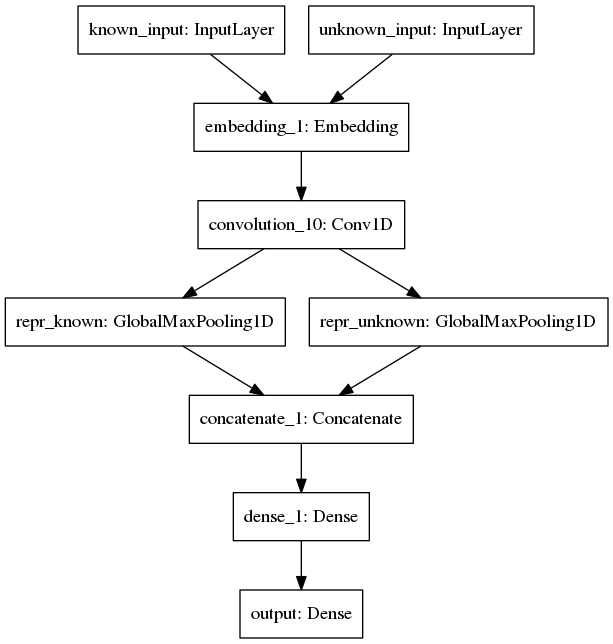
\includegraphics[width=0.8\textwidth]{./pictures/method/network1.png}
    \caption{Illustrate the structure of our first Siamese Neural Network
        Architecture.}
    \label{fig:network_1}
\end{figure}

The network obtained a validation accuracy of 0.68684. We have shown both the
training and validation accuracies in the different epochs in Figure
\ref{fig:network1_accuracies}. In that plot we can see that the network very
quickly overfits the training data and no longer learns anything general.

\begin{figure}[htb]
    \centering
    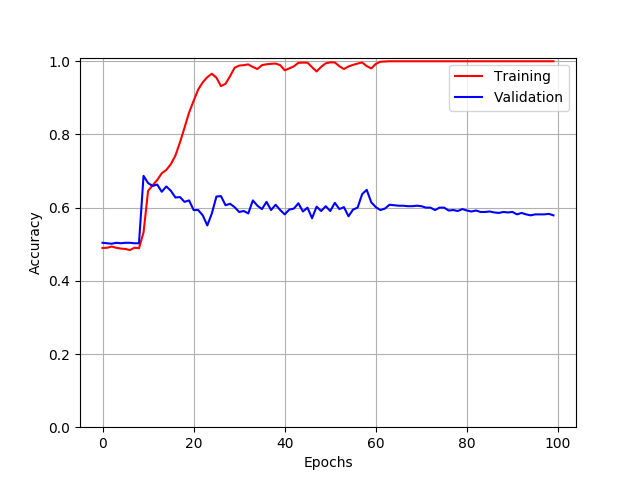
\includegraphics[width=0.5\textwidth]{./pictures/method/network_1_accuracies.png}
    \caption{Training and validation accuracies for the iteration 1 network in
        the different epochs of the networks execution.}
    \label{fig:network1_accuracies}
\end{figure}

Validation true positives 269

Validation true negatives 253

Validation false positives 109

Validation false negatives 129


\subsection{Siamese Neural Network - Iteration 2}

% TODO: Illustrate how dropout corresponds to training different subnetworks in
% each iteration.

In our last network we observed that the network after a few number of epochs
overfitted on the training dataset. The validation accuracy quickly began
stalling as the training accuracy went to 100\%. We therefore focused our
second network architecture on limiting overfitting. We added a dropout layer
before the output layer. A dropout layer is a layer that will randomly remove
neurons from a neural network during training. The layer prevents overfitting
by making sure that the network cannot rely on the output of all neurons during
training. This unpredictability makes it harder for the network to learn
specific quirks of the training dataset since small quirks will only be picked
up by a small amount of neurons while larger trends will be represented by a
larger set of neurons. \cite{JMLR:v15:srivastava14a} investigated the use of
dropout layers in different problem settings. They found that dropout layers
reduced overfitting in all problems they looked at. In particular they found
that document classification which is similar to what we are doing were also
improved. The main drawback of a dropout layer is that it increase the run time
of training the networks (\cite{JMLR:v15:srivastava14a}).

In iteration 1 the function we used to merge features from the known and unknown
text together were a concatenation. If we let the extracted features of the
known text be $K_i$ and the extracted features of the unknown text be $U_i$ then
$K_0$ and $U_0$ correspond to the same feature extracted from the two texts. The
concatenation merge function would then produce,

\begin{equation}
    merge(K, U) \rightarrow \left(
        K_0, K_1, \dots, K_n, U_0, U_1, \dots, U_n
    \right)^T.
\end{equation}

That means that the neural network would have to figure out by itself that input
$0$ were related in particular to input $n + 1$. To save the network that task
we also replaced the merging function to the absolute difference of the feature
vectors. That means that our merge function became,

\begin{equation}
    merge(K, U) \rightarrow \left(
        (|K_0 - U_0|), (|K_1 - U_1|), \dots, (|K_n - U_n|)
    \right)^T.
\end{equation}

So the network no longer has to learn arbitrary indexes. Instead it can learn
which features is important for authorship verification and learn thresholds for
when each feature is important. With the new merging we will have a large number
whenever the two features are far apart and a small number whenever they are
close to each other.

We changed the convolutional filters we used from 1000 convolutional filters of
size 10 to 500 convolutional filters of size 4 and 500 convolutional filters of
size 8. The idea was that the filters could learn different features where some
of the features would consist of a large number of characters and other of the
features would consist of a small number of characters. The architecture of our
network from iteration 2 is shown in Figure \ref{fig:network_2}.

\begin{figure}
    \centering
    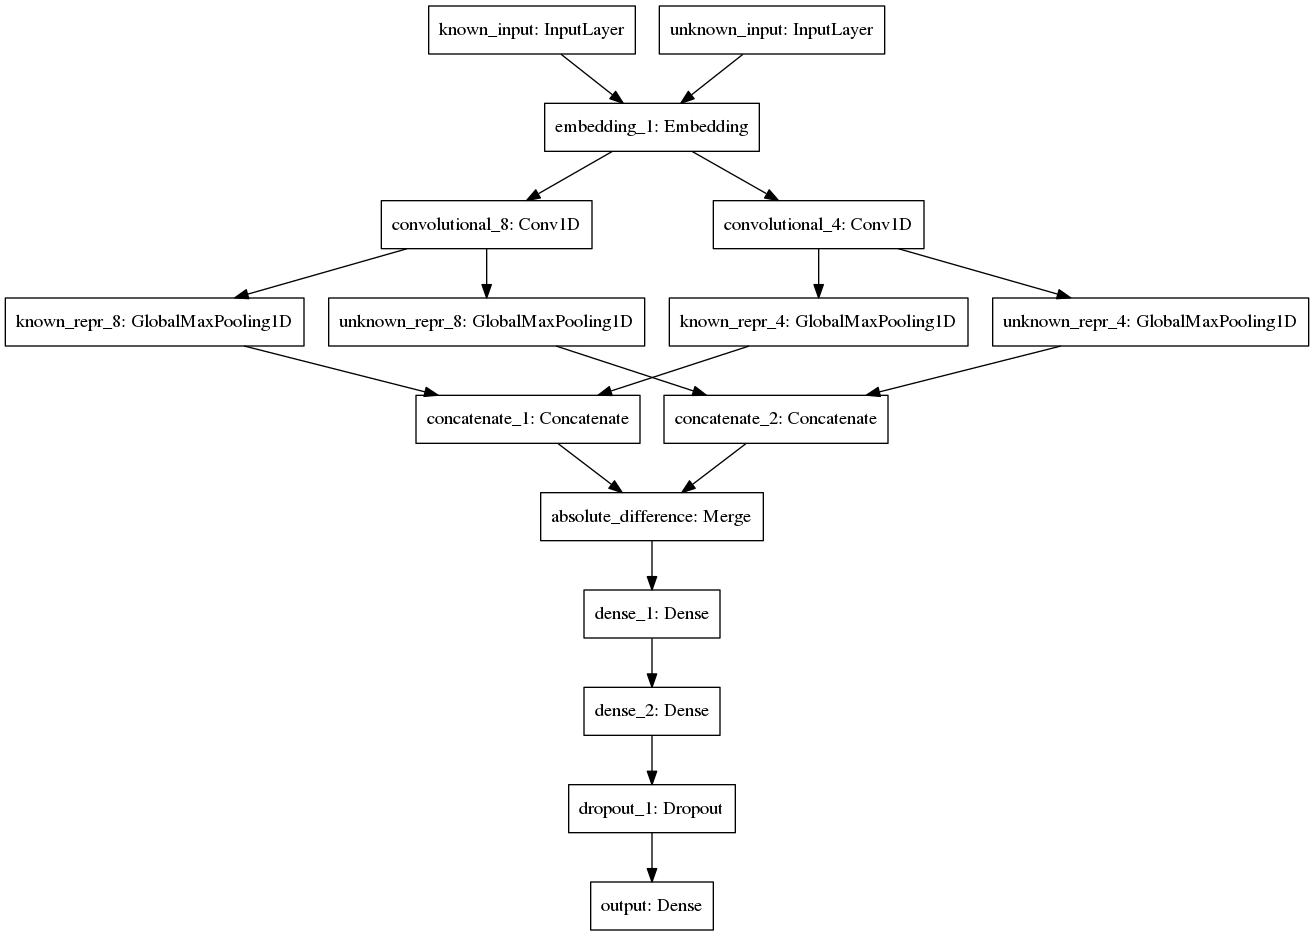
\includegraphics[width=\textwidth]{./pictures/method/network2.png}
    \caption{Illustrate the structure of our second Siamese Neural Network
        Architecture.}
    \label{fig:network_2}
\end{figure}

We also added more dense layers to the model. A plot of the
training and validation accuracies per epoch can be seen in Figure
\ref{fig:network2_accuracies}.

\begin{figure}
    \centering
    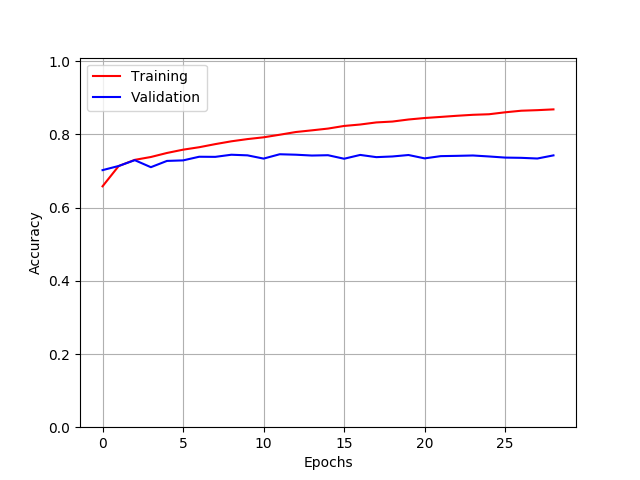
\includegraphics[width=0.5\textwidth]{./pictures/method/network_2_accuracies.png}
    \caption{Shows the training and validation accuracies on the second
        network.}
    \label{fig:network2_accuracies}
\end{figure}

The maximum validation accuracy obtained were 0.74464 in epoch 12.


TODO:
\begin{itemize}
    \item Use squared distance as merge function to get larger differences
        between close and far apart.
    \item Try to not use dense network but a distance metric (we didn't get to
        do that this week).
    \item Network 2 seem to not improve much after first epoch. Try to use a
        larger network and observe the effect.
    \item Use thresholding to manipulate the true positives (etc) and see what
        results we can get (also didn't do it this week).
    \item Look at learning rate of the network to make sure that the ReLu
        neurons don't die.
\end{itemize}
